
\documentclass[t]{beamer}
\usetheme[deutsch]{KIT}
\setbeamercovered{transparent}
\setbeamertemplate{navigation symbols}{}

\KITfoot{Tutoriumsmaterial von Alexander Kwiatkowski, Michael Vollmer und Matthias Holoch \hspace{2.5cm} Basierend auf den Folien von Simon Stroh und Moritz v. Looz}
\usepackage[utf8]{inputenc}
\usepackage{amsmath}
\usepackage{ifthen}
\usepackage{amssymb}
\usepackage{tikz}
\usepackage{ngerman}
\usepackage[normalem]{ulem}
\usetikzlibrary{automata}
\usenavigationsymbols


\title{Theoretische Grundlagen der Informatik}
\subtitle{Tutorium}
\author{Alexander Kwiatkowski, Michael Vollmer und Matthias Holoch}

\institute[IKS]{Institut für Kryptographie und Sicherheit}

\TitleImage[height=\titleimageht]{images/tmaschine.png}

\newcommand{\N}{\ensuremath{\mathbb{N}}}
\newcommand{\M}{\ensuremath{\mathcal{M}}}
\newcommand{\classP}{\ensuremath{\mathcal{P}}}
\newcommand{\classNP}{\ensuremath{\mathcal{NP}}}
\newcommand{\co}{\ensuremath{\mathsf{co\text{-}}}}
\newcommand{\pot}{\ensuremath{\mathcal{P}}}
\newcommand{\abs}[1]{\ensuremath{\left\vert #1 \right\vert}}
\newcommand{\menge}[2]{\ensuremath{\left\lbrace #1 \,\middle\vert\, #2 \right\rbrace}}
\newcommand{\ducttape}[1]{\vspace{#1}}
\newcommand{\neglit}[1]{\overline{#1\vphantom{x^a}}}
\newcommand{\recipe}{\raisebox{-.3cm}{
\includegraphics[scale=.15]{images/chefs-cap.png}}\hspace{0.2cm}}
\newcommand{\opt}[1]{\ensuremath{\text{OPT}(#1)}}
\newcommand{\A}[1]{\ensuremath{\mathcal{A}(#1)}}
\renewcommand{\O}[1]{\ensuremath{\mathcal{O}(#1)}}
\newcommand{\msout}[1]{\text{\sout{\ensuremath{#1}}}}

\newcommand{\invincible}{\setbeamercovered{invisible}} %  "Yesss! I am invincible!!" (Boris Grishenko)
\newcommand{\vincible}{\setbeamercovered{transparent}}
\renewcommand{\solution}[1]{\invincible \pause #1 \vincible}
\newcommand{\micropause}{\\[8pt]}

% \@ifundefined{tikzset}{}{\tikzset{initial text=}} % Text "start" bei Startknoten unterdrücken
\tikzstyle{every node}=[thick]
\tikzstyle{every line}=[thick]

\newcommand{\tutnr}[1]{
  \subtitle{Tutorium #1}
	\begin{frame}
		\maketitle
	\end{frame}
}

\newcommand{\uebnr}[1]{
  \subtitle{Anmerkungen zum #1. Übungsblatt}
	\begin{frame}
		\maketitle
	\end{frame}
}

\begin{document}

\newcommand{\start}[3]
{
  \draw (#1*2,#2*2) node{$#3$};
  \draw (#1*2,#2*2) circle(0.4cm);
  \draw [->] (#1*2-0.9,#2) -- (#1*2-0.4,#2);
}
\newcommand{\final}[3]
{
  \draw (#1*2,#2*2) node{$#3$};
  \draw (#1*2,#2*2) circle(0.4cm);
  \draw (#1*2,#2*2) circle(0.32cm);
}
\newcommand{\startfinal}[3]
{
  \draw (#1*2,#2*2) node{$#3$};
  \draw (#1*2,#2*2) circle(0.4cm);
  \draw (#1*2,#2*2) circle(0.32cm);
  \draw [->] (#1*2-0.9,#2) -- (#1*2-0.4,#2);
}
\newcommand{\state}[3]
{
  \draw (#1*2,#2*2) node{$#3$};
  \draw (#1*2,#2*2) circle(0.4cm);
}
\newcommand{\tol}[4]
{
  \draw (#1+#3,#2*2) node[above]{$#4$};
  \draw [->] (#1*2-0.4,#2*2) -- (#3*2+0.4,#2*2);
}
\newcommand{\tor}[4]
{
  \draw (#1+#3,#2*2) node[above]{$#4$};
  \draw [->] (#1*2+0.4,#2*2) -- (#3*2-0.4,#2*2);
}
\newcommand{\tot}[4]
{
  \draw (#1*2,#2+#3) node[right]{$#4$};
  \draw [->] (#1*2,#2*2+0.4) -- (#1*2,#3*2-0.4);
}
\newcommand{\tob}[4]
{
  \draw (#1*2,#2+#3) node[right]{$#4$};
  \draw [->] (#1*2,#2*2-0.4) -- (#1*2,#3*2+0.4);
}
\newcommand{\totl}[5]
{
  \draw (#1+#3,#2+#4) node[above right]{$#5$};
  \draw [->] (#1*2-0.283,#2*2+0.283) -- (#3*2+0.283,#4*2-0.283);
}
\newcommand{\totr}[5]
{
  \draw (#1+#3,#2+#4) node[above left]{$#5$};
  \draw [->] (#1*2+0.283,#2*2+0.283) -- (#3*2-0.283,#4*2-0.283);
}
\newcommand{\tobl}[5]
{
  \draw (#1+#3,#2+#4) node[below right]{$#5$};
  \draw [->] (#1*2-0.283,#2*2-0.283) -- (#3*2+0.283,#4*2+0.283);
}
\newcommand{\tobr}[5]
{
  \draw (#1+#3,#2+#4) node[below left]{$#5$};
  \draw [->] (#1*2+0.283,#2*2-0.283) -- (#3*2-0.283,#4*2+0.283);
}
\newcommand{\rloopl}[3]
{
  \draw (#1*2-1,#2*2) node[left]{$#3$};
  \draw [->] (#1*2-0.35,#2*2-0.2) arc (-30:-320:0.32cm);
}
\newcommand{\rloopr}[3]
{
  \draw (#1*2+1,#2*2) node[right]{$#3$};
  \draw [->] (#1*2+0.35,#2*2+0.2) arc (150:-140:0.32cm);
}
\newcommand{\rloopt}[3]
{
  \draw (#1*2,#2*2+1) node[above]{$#3$};
  \draw [->] (#1*2-0.2,#2*2+0.35) arc (240:-50:0.32cm);
}
\newcommand{\rloopb}[3]
{
  \draw (#1*2,#2*2-1) node[below]{$#3$};
  \draw [->] (#1*2+0.2,#2*2-0.35) arc (60:-230:0.32cm);
}
\newcommand{\lloopl}[3]
{
  \draw (#1*2-1,#2*2) node[left]{$#3$};
  \draw [->] (#1*2-0.35,#2*2+0.2) arc (30:320:0.32cm);
}
\newcommand{\lloopr}[3]
{
  \draw (#1*2+1,#2*2) node[right]{$#3$};
  \draw [->] (#1*2+0.35,#2*2-0.2) arc (-150:140:0.32cm);
}
\newcommand{\lloopt}[3]
{
  \draw (#1*2,#2*2+1) node[above]{$#3$};
  \draw [->] (#1*2+0.2,#2*2+0.35) arc (-60:230:0.32cm);
}
\newcommand{\lloopb}[3]
{
  \draw (#1*2,#2*2-1) node[below]{$#3$};
  \draw [->] (#1*2-0.2,#2*2-0.35) arc (-240:50:0.32cm);
}
\tutnr{2}

\section{Altlasten}
\subsection{Altlasten}

\begin{frame}
\frametitle{Automaten und ihre Fehlerzustände}
\begin{itemize}
	\item Ein vollständiger DEA benötigt einen expliziten Fehlerzustand.
	\item Ein DEA mit implizitem Fehlerzustand (alle nicht eingezeichneten Überführungen führen in den Fehlerzustand) heißt unvollständig.
	\item Ein NEA wird i.d.R. nicht vollständig dargestellt ($\Rightarrow$ also kann Fehlerzustand auch implizit sein)
\end{itemize}
\end{frame}

\begin{frame}
\frametitle{Wdh. Übungsblatt}
\begin{itemize}
	\item Jeder muss eine eigene Abgabe anfertigen
	\item Lerngruppen bis 5 Personen
	\item Letzte Aufgabe (mit Stern) wird nicht gewertet
\end{itemize}
\end{frame}

\section{Semi-Thue-Systeme}
\subsection{Semi-Thue-Systeme}

\begin{frame}
\frametitle{Semi-Thue-Systeme}
Ein Semi-Thue-System besteht aus
\begin{itemize}
	\item einem nichtleeren Alphabet $A$
\end{itemize}
und
\begin{itemize}
	\item einer Produktionsmenge $P \subset \{A^* \rightarrow A^*\}$
\end{itemize}~\\
Beispiel:~\\
$A = \{a, b, c\}$~\\
$P = \{ab \rightarrow c, bc \rightarrow a, aa \rightarrow \lambda, cc \rightarrow \lambda\}$~\\~\\
Beispieleingaben:
\begin{description}
	\item[abc] $\Rightarrow$ cc $\Rightarrow$ $\lambda$~\\
	$\Rightarrow$ aa $\Rightarrow$ $\lambda$~\\
	\item[aab] $\Rightarrow$ b~\\
	$\Rightarrow$ ac
\end{description}
Produktionen sind nicht immer eindeutig.
\end{frame}

\section{Äquivalenzklassen}
\subsection{Äquivalenzklassen}
\begin{frame}
	\frametitle{Äquivalenzklassen}
	\begin{block} {Äquivalenz}
		\begin{itemize}
			\item Zwei Zustände sind äquivalent, wenn es für das Erreichen eines Endzustandes durch Abarbeiten eines Wortes $w$ unerheblich ist, aus welchem der beiden Zustände wir starten.
		\end{itemize}
	\end{block}
	\begin{block} {Definition}
  Zwei Zustände $p$ und $q$ eines deterministischen endlichen Automaten heißen \emph{äquivalent} ($p \equiv q$),
  wenn für alle Wörter $w\in\Sigma^*$ gilt:
  \[
   \delta(p, w)\in F \Leftrightarrow \delta(q, w)\in F
  \]
  Offensichtlich ist $\equiv$ eine Äquivalenzrelation. Mit $[p]$ bezeichnen wir die \emph{Äquivalenzklasse} der zu $p$ äquivalenten Zustände.
  \end{block}
\end{frame}

\subsection{Aufgabe 1}
\begin{frame}
	\frametitle{Aufgabe 1}
		Gegeben sei der folgende endliche Automat:\\
		$\mathcal{M} = (\mathcal{Q},\Sigma,\delta,s_0,\mathcal{F})$ mit
		$\mathcal{Q} = \{s_0,s_1,s_2,s_3,s_4\}, \Sigma = \{0,1\}, \mathcal{F} = \{s_4\}$
		und $\delta$ gegeben durch:
	\begin{center}
		\resizebox{4.5cm}{!} {%
		\begin{tikzpicture}[line width=1pt]
			\start{0}{0}{s_0}
			\totr{0}{0}{1}{1}{0}
			\tor{0}{0}{1}{1}
			\state{1}{1}{s_1}
			\tor{1}{1}{2}{0}
			\tob{1}{1}{0}{1}
			\state{1}{0}{s_2}
			\tor{1}{0}{2}{0}
			\rloopb{1}{0}{1}
			\state{2}{0}{s_3}
			\tot{2}{0}{1}{0}
			\draw [->] (4,-0.4) arc (0:-180:2cm);
			\draw (2,-2.4) node[below]{$1$};
			\final{2}{1}{s_4}
			\rloopr{2}{1}{0,1}
		\end{tikzpicture}%
		}
	\end{center}
	\begin{enumerate}
		\item Ist der gegebene endliche Automat deterministisch?
		\item Zeichnen Sie den Äquivalenzklassenautomaten!
		\item Geben Sie die Äquivalenzklassen der Zustände vom entstandenen Automaten an!
	\end{enumerate}
\end{frame}

\section{Minimierung}
\subsection{Minimierung}

\begin{frame}
\frametitle{Automatenminimierung}
\begin{itemize}
	\item Schritt 1: nicht erreichbare Zustände entfernen
	\item Schritt 2: Liste mit Paaren von Zuständen erstellen (Matrixform)
	\item Schritt 3: Alle Paare, die einen akzeptierenden und einen nicht-akzeptierenden enthalten entfernen (bzw. eine 1 in die Matrix schreiben)
	\item Schritt 4: Alle Paare bei denen es eine Eingabe gibt, sodass das Paar der resultierenden Zustände bereits entfernt wurde und das Paar nicht zweimal den selben Zustand enthält, entfernen~\\
	Formal:
	\begin{multline*}
	\forall (q_i q_j) \in F \text{ mit } (\delta(q_i, w), \delta(q_j, w)) \notin F \land \delta(q_i, w) \neq \delta(q_j, w)\}:\\
	\text{Entferne } (q_i, q_j) \text{ aus F}
	\end{multline*}
	\item Schritt 5: Wiederhole Schritt 4 bis nichts mehr entfernt wird.
	\item Schritt 6: Leere Felder in der Matrix zeigen welche Zustände die selbe Äquivalenzklasse haben
\end{itemize}
\end{frame}

\subsection{Aufgabe 3}
\begin{frame}
	\frametitle{Aufgabe 3}
	Gegeben sei der folgende deterministische endliche Automat:\\
	$\mathcal{M} = (\mathcal{Q},\Sigma,\delta,q_0,\mathcal{F})$ mit
	$\mathcal{Q} = \{q_0,q_1,q_2,q_3,q_4,q_5\}, \Sigma = \{0,1\}, \mathcal{F} =
	\{q_3,q_5\}$ und $\delta$ gegeben durch:
	\begin{center}
		\resizebox{5.5cm}{!} {%
		\begin{tikzpicture}[line width=1pt]
			\start{0}{0}{q_0}
			\tobr{0}{0}{1}{-1}{0}
			\tor{0}{0}{1}{1}
			\state{1}{0}{q_1}
			\tor{1}{0}{2}{0}
			\rloopt{1}{0}{1}
			\state{2}{0}{q_2}
			\tor{2}{0}{3}{0}
			\final{3}{0}{q_3}
			\rloopt{3}{0}{1}
			\state{1}{-1}{q_4}
			\tor{1}{-1}{2}{0}
			\final{2}{-1}{q_5}
			\draw (5,-1) node[below right]{$1$};
			\draw [->] (4.283,-1.717) -- (5.717,-0.283);
		\end{tikzpicture}%
		}
	\end{center}
	\begin{enumerate}
		\item Vervollständigen Sie den Automaten, d.h. führen Sie einen Fehlerzustand ein!
		\item Minimieren Sie den vervollständigten Automaten!
	\end{enumerate}
\end{frame}

\section{Potenzmengenkonstruktion}
\subsection{Eliminierung von $\lambda$-Übergängen}
\begin{frame}
	\frametitle{Eliminierung von $\lambda$-Übergängen}
	\begin{block}{Allgemein}
	\begin{itemize}
	 \item Zu jedem nichtdeterministischen endlichen Automaten mit $\lambda$-Übergängen gibt es einen äquivalenten nichtdeterministischen
	 endlichen Automaten ohne $\lambda$-Übergänge, der nicht mehr Zustände hat.
	 \item Äquivalent heißt, er akzeptiert die selbe Sprache.
	\item Der $\lambda$-Abschluss $E(q)$ eines Zustandes $q$ ist definiert als die Menge aller Zustände, die von $q$ aus durch lediglich $\lambda$-Übergänge erreichbar sind ($q$ selbst zählt auch dazu).
	\end{itemize}
	\end{block}
\end{frame}
\begin{frame}
\frametitle{Eliminierung von $\lambda$-Übergängen}
	\begin{block}{Konstruktion}
	Zu einem NEA \(A := (Q, \Sigma, \delta, s, F)\) mit $\lambda$-Übergängen konstruieren wir einen 
	  äquivalenten NEA \(\tilde{A} := (\tilde{Q}, \Sigma, \tilde{\delta}, \tilde{s}, \tilde{F})\) mit
	 \begin{itemize}
	 \item gleicher Zustandsmenge \(\tilde{Q} := Q\)
	 \item gleichem Startzustand \(\tilde{s} := s\)
	 \item neuer Endzustandsmenge \(\tilde{F} := \menge{q \in Q}{E(q)\cap F \neq \emptyset}\)
	 \begin{itemize}
	 	\item ``alle Zustände, in deren $\lambda$-Abschluss ein Endzustand liegt''
	 \end{itemize}
	 \item neuer Übergangsfunktion $\tilde{\delta}(q,a) := 
	 \begin{cases}
	  \{q\}			& \text{falls $a = \lambda$} \\
	 \delta(E(q),a)	& \text{sonst}
	 \end{cases}$
	 \end{itemize}
	\end{block}
	\begin{block}{Eigenschaften von \(\tilde{A}\)}
	 \(L(\tilde{A}) = L(A)\) und \(|\tilde{Q}| = |Q|\).
	\end{block}

\end{frame}

\subsection{Potenzmengenkonstruktion}

\frame{
\frametitle{Potenzmengenkonstruktion}
Zu jedem nichtdeterministischen endlichen Automaten existiert ein äquivalenter deterministischer endlicher Automat.
 \begin{figure}[H]
 \begin{center}
 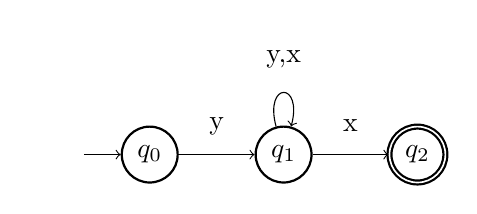
\begin{tikzpicture}[node distance=1.7cm]
 \tikzstyle{every node}=[circle, thick, minimum size = 7mm]
 \tikzstyle{normal}=[draw]
 \node[normal] 	(q0)		{$q_0$};
 \node[normal] 	(q1)	[right of=q0] {$q_1$};
 \node[normal,double]		(q2)	[right of=q1]{$q_2$};
 \node 		(s) 	[left of =q0, xshift=0.5cm]	{};
 
 \draw[->](s) to (q0);
 \draw[->](q0) to node[above]{y} (q1);
 \draw[->, loop above](q1) to node[above]{y,x} (q1);
 \draw[->](q1) to node[above]{x} (q2);x
 \end{tikzpicture}
 \end{center}
 \end{figure}
In eine Tabelle werden die Automatenzustände und ihre Folgezustände bei jeweiliger Eingabe eingetragen. \\
\begin{center}
\vspace{-6pt}
\begin{tabular}{l|l|l}
    & y & x \\
\hline
 $\{q_0\}$ 	&	 $\{q_1\}$	&	$\emptyset$ \\
 $\{q_1\}$	&	$\{q_1\}$	&	$\textcolor{red}{\{q_1, q2 \}}$\\
\end{tabular}
\end{center}
}
\frame{
\frametitle{Potenzmengenkonstruktion}
Ein \textcolor{red}{neuer Zustand} entsteht, wenn man von einem alten Zustand durch eine Eingabe in mehrere Zustände kommt.
\vspace{-0.3cm}
\begin{center}
\begin{tabular}{l|l|l}
    & y & x \\
\hline
 $\{q_0\}$ 	&	 $\{q_1\}$	&	$\emptyset$ \\
 $\{q_1\}$	&	$\{q_1\}$	&	$\textcolor{red}{\{q_1, q_2\}}$\\
 $\textcolor{red}{\{q_1, q_2\}}$ & 	$\{q_1\}$	&	$\{q_1, q_2\}$\\
 $\emptyset$	&	$\emptyset$		& 	$\emptyset$
\end{tabular}
\end{center}
\vspace{-1cm}
\begin{figure}[H]
\begin{center}
 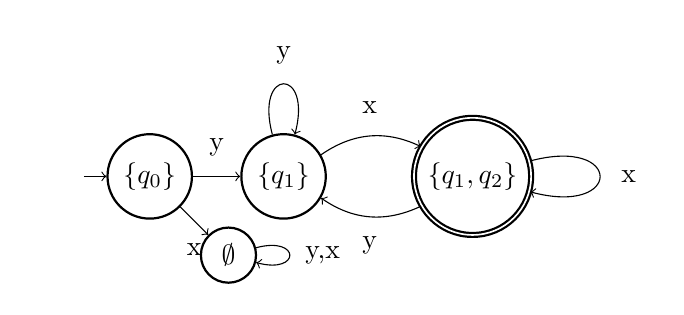
\begin{tikzpicture}[node distance=1.7cm]
 \tikzstyle{every node}=[circle, thick, minimum size = 7mm]
 \tikzstyle{normal}=[draw]
 \node[normal] 	(q0)		{\{$q_0$\}};
 \node[normal] 	(q1)	[right of=q0] {\{$q_1$\}};
 \node[normal,double,node distance=2.4cm]		(q2)	[right of=q1]{\{$q_1, q_2$\}};
 \node[normal]	(f) at (1,-1)	{$\emptyset$};
 \node 		(s) 	[left of =q0, xshift=0.5cm]	{};
  \draw[->](q0) to node[above]{y}(q1);
  \draw[->](s) to (q0);
  \draw[->](q0) to node[below]{x}(f);
  \draw[->,loop above](q1) to node[above]{y}(q1);
  \draw[->,bend left](q1) to node[above]{x}(q2);
  \draw[->, bend left](q2) to node[below]{y}(q1);
  \draw[->, loop right](q2) to node[right]{x}(q2);
  \draw[->, loop right](f) to node[right]{y,x}(f);
\end{tikzpicture}
\end{center}
\end{figure}
}
\frame{
\frametitle{Potenzmengenkonstruktion}
Die Einträge der ersten Spalte sind die neuen Zustände. Alle Mengen, die einen Endzustand enthalten, sind wiederum im neuen Automaten Endzustände.
\begin{figure}[H]
\begin{center}
 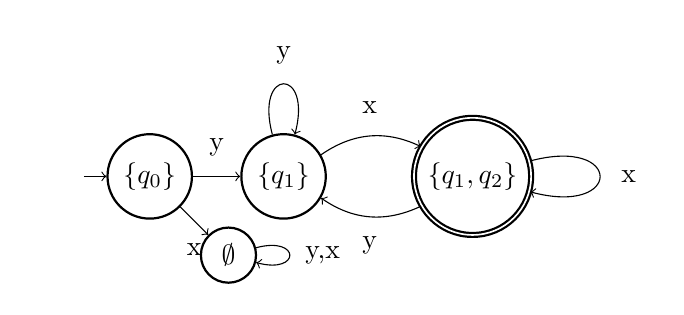
\begin{tikzpicture}[node distance=1.7cm]
 \tikzstyle{every node}=[circle, thick, minimum size = 7mm]
 \tikzstyle{normal}=[draw]
 \node[normal] 	(q0)		{\{$q_0$\}};
 \node[normal] 	(q1)	[right of=q0] {\{$q_1$\}};
 \node[normal,double,node distance=2.4cm]		(q2)	[right of=q1]{\{$q_1, q_2$\}};
 \node[normal]	(f) at (1,-1)	{$\emptyset$};
 \node 		(s) 	[left of =q0, xshift=0.5cm]	{};
  \draw[->](q0) to node[above]{y}(q1);
  \draw[->](s) to (q0);
  \draw[->](q0) to node[below]{x}(f);
  \draw[->,loop above](q1) to node[above]{y}(q1);
  \draw[->,bend left](q1) to node[above]{x}(q2);
  \draw[->, bend left](q2) to node[below]{y}(q1);
  \draw[->, loop right](q2) to node[right]{x}(q2);
  \draw[->, loop right](f) to node[right]{y,x}(f);
\end{tikzpicture}
\end{center}
\end{figure}
}

\subsection{Aufgabe 2}
\begin{frame}
	\frametitle{Aufgabe 2}
	Gegeben sei ein nichtdeterministischer endlicher Automat (NEA):\\
	$\mathcal{M} = (\mathcal{Q},\Sigma,\delta,q_0,\mathcal{F})$ mit
	$\mathcal{Q} = \{q_0,q_1,q_2\}, \Sigma = \{a,b\}, \mathcal{F} = \{q_2\}$
	und $\delta$ gegeben durch:
	\begin{center}
		\resizebox{4.5cm}{!} {%
		\begin{tikzpicture}[line width=1pt]
			\start{0}{0}{q_0}
			\tor{0}{0}{1}{a}
			\state{1}{0}{q_1}
			\rloopt{1}{0}{a,b}
			\tor{1}{0}{2}{b}
			\final{2}{0}{q_2}
		\end{tikzpicture}%
		}
	\end{center}
	\begin{enumerate}
		\item Geben Sie einen entsprechenden deterministischen endlichen Automaten
		(DEA) an, der die gleiche\\
		Sprache akzeptiert! Benutzen Sie hierbei das Potenzmengenkonstruktionsverfahren!
		\item Ist der entstandene Automat vollständig? Wenn nicht, wie kann man den
		Automaten vervollständigen?\\
		Welche Mengen stellen bei dem Potenzmengenkonstruktionsverfahren einen
		Fehlerzustand dar?
	\end{enumerate}
\end{frame}

\subsection{Aufgabe 4}
\begin{frame}
	\frametitle{Aufgabe 4}
	Gegeben seien die folgenden beiden nichtdeterministischen endlichen Automaten:
	\begin{center}
		\resizebox{6.5cm}{!} {%
		\begin{tikzpicture}[line width=1pt]
			\startfinal{0}{0}{q_1}
			\rloopt{0}{0}{a}
			\draw [->] (0.4,0) arc (90:-90:1cm);
			\draw (1.4,-1) node[right]{$a,b$};
			\state{0}{-1}{q_2}
			\tot{0}{-1}{0}{b}
			\start{2}{0}{s_1}
			\tor{2}{0}{3}{\varepsilon}
			\tob{2}{0}{-1}{a}
			\final{3}{0}{s_2}
			\draw [->] (6,0.4) arc (0:180:1cm);
			\draw (5,1.4) node[above]{$a$};
			\state{2}{-1}{s_3}
			\draw (5,-1) node[below right]{$a,b$};
			\draw [->] (4.283,-1.717) -- (5.717,-0.283);
			\rloopb{2}{-1}{b}
		\end{tikzpicture}%
		}
	\end{center}
	Wandeln Sie diese mittels des Potenzmengenkonstruktionsverfahrens in
	deterministische endliche Automaten um!
\end{frame}

\section{Schluss}
\subsection{Schluss}

\begin{frame}
\frametitle{Bis zum nächsten Mal!}
\vspace{0.3cm}
\begin{center}
	\resizebox{11.85cm}{!} {%
	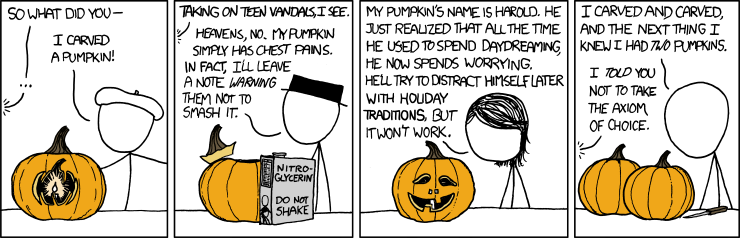
\includegraphics[height=0.8\textheight]{images/xkcd_804.png}%
	}
\end{center}
\end{frame}

\frame{
  \frametitle{Lizenzen}
  \center
  
\includegraphics[width=2em]{images/by}
  
\includegraphics[width=2em]{images/cc}
  
\includegraphics[width=2em]{images/sa}
  \\
  {\tiny

Dieses Werk ist unter einem ``Creative Commons Namensnennung-Weitergabe unter gleichen Bedingungen 3.0 Deutschland``-Lizenzvertrag lizenziert. Um eine Kopie der Lizenz zu erhalten, gehen Sie bitte zu \href{http://creativecommons.org/licenses/by-sa/3.0/de/}{http://creativecommons.org/licenses/by-sa/3.0/de/} oder schreiben Sie an Creative Commons, 171 Second Street, Suite 300, San Francisco, California 94105, USA.\\
  \vspace{1cm}
  Davon ausgenommen sind das Titelbild, welches aus der März-April 2002 Ausgabe von American Scientist erschienen ist und ohne Erlaubnis verwendet wird, sowie das KIT Beamer Theme. Hierfür gelten die Bestimmungen der jeweiligen Urheber.
  \vspace{1cm}
  \\ 
  }
  %Habe hier die Reihenfolge etwas umgestellt, weil die Formatierung bei mir komisch aussah. 
  %Wenn es bei dir anders ist, kannst du es auch wieder zurückändern, dann haben wir unterschiedliche Kompilieroptionen
}

\end{document}
